\documentclass[11pt]{article}
\usepackage[margin=1.15in]{geometry}
\usepackage[T1]{fontenc}
\usepackage{lmodern}
\usepackage{amsmath,amssymb,amsthm,mathtools}
\usepackage{booktabs}
\usepackage{graphicx}
\usepackage[normalem]{ulem}
\usepackage[dvipsnames]{xcolor}
\usepackage[numbers,sort&compress]{natbib}
\usepackage{microtype}
\usepackage{enumitem}
\usepackage{placeins}
\usepackage[font=small,labelfont=bf,labelsep=period,skip=6pt]{caption}
\usepackage[colorlinks=true,linkcolor=MidnightBlue,citecolor=MidnightBlue,urlcolor=MidnightBlue]{hyperref}
\usepackage[capitalise,noabbrev]{cleveref}

\setlength{\emergencystretch}{1.5em}
\renewcommand{\topfraction}{0.9}
\renewcommand{\bottomfraction}{0.8}
\renewcommand{\textfraction}{0.1}
\renewcommand{\floatpagefraction}{0.75}

\theoremstyle{plain}
\newtheorem{theorem}{Theorem}
\newtheorem{proposition}[theorem]{Proposition}
\newtheorem{lemma}[theorem]{Lemma}
\newtheorem{corollary}[theorem]{Corollary}
\theoremstyle{definition}
\newtheorem{definition}[theorem]{Definition}
\theoremstyle{remark}
\newtheorem{remark}[theorem]{Remark}
\newtheorem*{question}{Question}

\newcommand{\N}{\mathbb{N}}
\newcommand{\R}{\mathbb{R}}
\newcommand{\Sym}{\mathrm{S}}
\newcommand{\Alt}{\mathrm{A}}
\newcommand{\row}{\mathrm{H}}
\DeclarePairedDelimiter{\abs}{\lvert}{\rvert}
\DeclarePairedDelimiter{\ceil}{\lceil}{\rceil}

\newcommand{\NumCells}{51}
\newcommand{\NumImproved}{33}
\newcommand{\NumMatched}{18}
\newcommand{\NumWorse}{0}
\newcommand{\MeanGain}{18.5}
\newcommand{\MaxGain}{39.4}
\newcommand{\TopCell}{$12\times13$}
\newcommand{\TopOld}{274.0}
\newcommand{\TopNew}{166.0}
\newcommand{\NumImprovedOneMin}{33}
\newcommand{\NumBudgetCells}{35}
\newcommand{\BudgetOneMin}{13.3}
\newcommand{\BudgetFiveMin}{15.8}
\newcommand{\BudgetTenMin}{16.8}
\newcommand{\NumTimingRuns}{165}
\newcommand{\NumSeeds}{5}
\newcommand{\AllReached}{all}
\newcommand{\MedianBeat}{0.12}
\newcommand{\MaxBeat}{143}
\newcommand{\NumCellsUnderOneSec}{23}
\newcommand{\NumCellsUnderOneMin}{33}
\newcommand{\MaxCellMedian}{54}
\newcommand{\MaxMatch}{0.07}
\newcommand{\MinSpeedupSAT}{43{,}636}


\title{\bfseries Leaving the Cyclic Orbit:\\[2pt]
\large Local Search, Exact Search and a Cubic Law for Balanced Latin Rectangles}
\author{Zhengyu Li\thanks{Georgia Institute of Technology. \texttt{brian.li@gatech.edu}}
  \and Vijay Ganesh\thanks{Georgia Institute of Technology. \texttt{vganesh45@gatech.edu}}}
\date{}

\begin{document}
\maketitle

\begin{abstract}
\noindent
Write a $k\times n$ Latin rectangle as $n$ points in the grid $[n]^k$, one point per symbol,
whose coordinates are the columns the symbol occupies. The rectangle is \emph{balanced} when
these points are pairwise equidistant in the $\ell_1$ metric, and its \emph{imbalance}
measures how far it is from that ideal. We study the minimum imbalance from three sides.
\emph{Constructively}, a simulated annealing that moves symbols within rows and only penalises
column clashes improves \NumImproved{} of the \NumCells{} best known values for $8\le n\le 13$,
by up to \MaxGain\%, and matches the rest.
We explain why earlier column-based local search could not find these rectangles. Every
column operation preserves a permutation group attached to the rectangle, its
\emph{row group}. For cyclic rectangles this group has order at most $n$, while
32 of our 33 new rectangles have row group $\Alt_n$ or $\Sym_n$.
\emph{Exactly}, a short branch and bound proves that the minimum imbalance of a $3\times 9$
rectangle is $56$, a value found by Díaz et al.\ whose optimality was open, and independently confirms the known optima for $3\times8$ and $4\times8$.
\emph{Asymptotically}, a pigeonhole argument in $[n]^k$ shows that for every fixed $k$ the minimum
imbalance grows like $n^3$. For $k=2$ the limit of $\min I/n^3$ exists, is attained by a permuton, and lies
between $4/375$ and about $0.120$. Along the way we observe that perfect balance is an $\ell_1$-equilateral problem, so
it forces $k=\Omega(n/\log n)$ rows.
For $2\times n$ rectangles, single two-minute annealing runs improve five of the seven six-hour MIP
upper bounds for $14\le n\le 20$.
\end{abstract}

\section{Introduction}

In an agricultural field trial, treatments are laid out on a grid of plots. When some pairs of
treatments are systematically planted closer together than others, spatial correlation in the
soil can bias their comparison~\citep{vanEs1993}. Latin designs remove the row and column
effects, but not this one. \emph{Spatially balanced} Latin squares ask, in addition, that every
pair of treatments be equally far apart on average~\citep{GomesSellmann2004,LeBrasGomesSelman2012}.
\citet{DiazLeBrasGomes2017} posed the same question for $k\times n$ rectangles, observed that
perfect balance is then usually impossible, and asked instead for rectangles of minimum
\emph{imbalance}. Since then the problem has driven work on SAT encodings that prove optima with checkable
proof certificates~\citep{RamaswamySzeider2023}, mixed-integer programming~\citep{MirkaEtAl2023},
streamliners written by large language models~\citep{VoborilRamaswamySzeider2025} and LLM agents
that reformulate models~\citep{VoborilSzeider2026}, and balanced Latin squares have served as a
test case for agentic neurosymbolic discovery~\citep{XiaEtAl2026}. The reference table
of~\citet{VoborilRamaswamySzeider2025}, which collects the best values obtained by all of these
approaches, is the starting point of this paper.

Here is the point of view of this paper. Record, for each symbol $u$, the columns
$c_1(u),\dots,c_k(u)$ that it occupies in the $k$ rows. This gives a point
$x_u\in[n]^k$, and the distance between two symbols used throughout the literature is exactly
the $\ell_1$ distance $\lVert x_u-x_v\rVert_1$. A balanced rectangle is therefore a set of $n$
points in a $k$-dimensional grid that are pairwise \emph{equidistant} in the taxicab metric.
The picture organises the whole paper. When $k$ is small compared with $n$, the grid is too
crowded for equidistance, and \cref{sec:cubic} makes this quantitative. When $k=n$ there is
room, consistent with the existence of balanced squares for infinitely many $n$. And it
suggests a search that moves individual points, rather than one that rearranges a rigid
algebraic pattern.

\paragraph{Contributions.}
\begin{enumerate}[leftmargin=*,itemsep=2pt]
\item \textbf{A relaxed local search} (\cref{sec:search}). Rows are kept as permutations, the
column condition becomes a penalty with an adaptive weight, and a move swaps two symbols
within a row. A move is evaluated exactly in $O(n)$ time. Against the reference table of
\citet{VoborilRamaswamySzeider2025}, the search improves \NumImproved{} of \NumCells{}
instances and matches the other \NumMatched{} (\cref{sec:results}).

\item \textbf{The row group} (\cref{sec:orbit}). We attach to each rectangle the permutation group
generated by the ratios of its rows. Column operations leave this group unchanged, so local
search that permutes columns of a cyclic rectangle~\citep{SmithGomesFernandez2005,DiazLeBrasGomes2017}
stays among rectangles whose row group has order at most $n$. For 32 of our 33 improved
rectangles the row group is the full alternating or symmetric group.

\item \textbf{A new optimum} (\cref{sec:exact}). A branch and bound that places one symbol at a
time proves that the known value $56$ is optimal for $3\times 9$, which was open, and independently reproduces the
known optima for $2\times n$ with $n\le 11$ and for $3\times 8$ and $4\times 8$.

\item \textbf{A cubic law} (\cref{sec:cubic}). For every fixed $k$, the minimum imbalance is
$\Theta(n^3)$, with the explicit lower constant $c_k=\max_m k\,m^{-k}(\frac13-\frac1m)$.
Perfect balance also requires $n\le e(\ell_1^k)=O(k\log k)$, by a classical bound on
equilateral sets.

\item \textbf{The case $k=2$} (\cref{sec:two}). On the open instances $14\le n\le 20$, a
single-seed two-minute annealing run improves the six-hour upper bounds of \citet{MirkaEtAl2023} for
$15\le n\le19$, ties at $n=14$ and is worse at $n=20$. Near-optimal
$2\times n$ rectangles look like a few broken diagonals, and the normalised imbalance appears to
stay near $0.11\,n^3$ up to $n=64$, which suggests a limit of about $0.12$. The limit exists and is the minimum of a continuous functional
on permutons.
\end{enumerate}

None of the algorithmic ingredients is new by itself. Simulated
annealing~\citep{KirkpatrickGelattVecchi1983}, row-preserving swaps with temporarily
violated column constraints~\citep{ZhangMa2008,XieEtAl2024} and adaptive penalties
(strategic oscillation~\citep{GloverHao2011}) are all established. What we add is their
combination for this objective and the row-group explanation of why it reaches rectangles that
earlier local search could not.

\section{Preliminaries}\label{sec:prelim}

A $k\times n$ \emph{Latin rectangle} ($k\le n$) is an array with entries in
$[n]=\{1,\dots,n\}$ in which no symbol repeats in a row or in a column. Let $c_i(u)$ denote the
column of symbol $u$ in row $i$ and $x_u=(c_1(u),\dots,c_k(u))\in[n]^k$. Following
\citet{DiazLeBrasGomes2017} and \citet{RamaswamySzeider2023},
\[
  d(u,v)=\sum_{i=1}^k\abs{c_i(u)-c_i(v)}=\lVert x_u-x_v\rVert_1,
  \qquad
  I(L)=\sum_{1\le u<v\le n}\abs[\big]{d(u,v)-t},
  \qquad t=\frac{k(n+1)}{3}.
\]
Each row contributes $\sum_{u<v}\abs{c_i(u)-c_i(v)}=\binom{n+1}{3}$ to the total distance, so
$t$ is the \emph{average} distance over all $\binom n2$ pairs. In particular the deviations
$d(u,v)-t$ sum to zero, and
\begin{equation}\label{eq:half}
  I(L)=2\sum_{u<v}\bigl(t-d(u,v)\bigr)^+ .
\end{equation}
Imbalance is therefore caused by the pairs that are too close. This one-line identity is the
engine of \cref{sec:cubic}. The quantity $3I$ is an integer, and as in the literature we write
imbalances as $x.0$, $x.3$ and $x.6$ for $x$, $x+\frac13$ and $x+\frac23$.

\paragraph{Two dictionaries.} A rectangle can be read through its rows or through its points.
Through its rows it is a $k$-tuple $(r_1,\dots,r_k)$ of bijections $r_i\colon[n]\to[n]$ from
columns to symbols, with $r_i(j)\ne r_{i'}(j)$ for $i\ne i'$. Through its points it is a set
$\{x_u\}$ in $[n]^k$ whose coordinate projections are bijections and in which every point has
distinct coordinates. The column condition says exactly that.
The imbalance is invariant under relabelling symbols and permuting rows, but not under
permuting columns. Relabelling symbols, we may assume $r_1=\mathrm{id}$.

\begin{figure}[t]
\centering
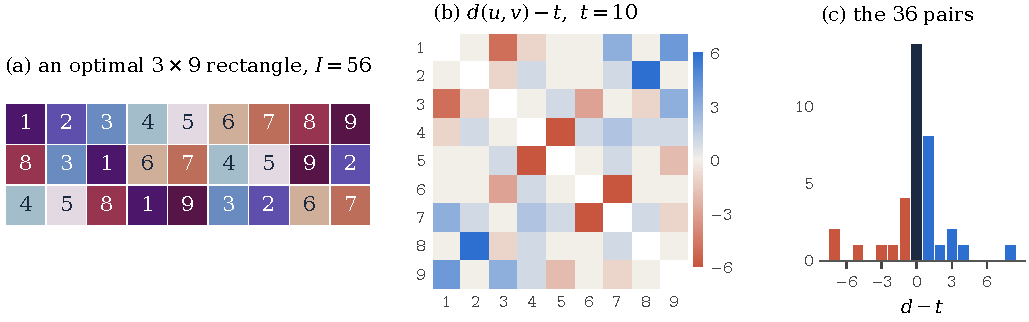
\includegraphics[width=\linewidth]{figures/optimum3x9.pdf}
\caption{A $3\times 9$ rectangle of imbalance $56$, which \cref{thm:3x9} proves optimal.
(a)~The rectangle, one colour per symbol. (b)~The deviation $d(u,v)-t$ of every pair from the
average distance $t=10$. Blue pairs are too far apart and red pairs too close. (c)~Histogram of
the $36$ deviations. They sum to zero, and $I=\sum\abs{d-t}=56$.}
\label{fig:optimum}
\end{figure}

\section{Search: rows as permutations, columns as a penalty}\label{sec:search}

The state of the search is a $k$-tuple of permutations with $r_1=\mathrm{id}$. It need not be
Latin. A \emph{move} picks a row $i\ge2$ and two columns $j_1\ne j_2$, and swaps the symbols
$a=r_i(j_1)$ and $b=r_i(j_2)$. In the point picture, the move exchanges the $i$-th coordinates of
the two points $x_a$ and $x_b$, and nothing else moves.

\begin{lemma}[Incremental evaluation]\label{lem:delta}
After the move, only the $2(n-2)$ distances $d(a,w)$ and $d(b,w)$ with $w\notin\{a,b\}$ change,
and with $p=c_i(w)$,
\[
  d'(a,w)=d(a,w)-\abs{j_1-p}+\abs{j_2-p},\qquad
  d'(b,w)=d(b,w)-\abs{j_2-p}+\abs{j_1-p}.
\]
Hence the exact change of $3I$ is computable in $O(n)$ integer operations.
\end{lemma}

\begin{proof}
Only the $i$-th coordinates of $x_a$ and $x_b$ change, and they are exchanged, so $d(a,b)$ is
unchanged and every other pair not containing $a$ or $b$ is untouched.
\end{proof}

\paragraph{Penalty.} Let $V$ be the number of excess occurrences of symbols in columns. It is
maintained in $O(1)$ per move with per-column counters. The search minimises $3I+W\cdot V$ and
records only states with $V=0$. Every $2^{16}$ proposals the weight $W$ is multiplied by
$1.02$ if the current state has conflicts and by $0.99$ otherwise, and it is kept in
$[1,4n^2]$, starting from $W=k$. The search can therefore leave the Latin rectangles, pass through
non-Latin states and come back. Moves that permute whole columns never leave the Latin
rectangles, and as \cref{sec:orbit} shows, they never change the row group.

\paragraph{Schedule.} The search starts from the cyclic rectangle $r_i(j)=i+j \bmod n$. It accepts
a move of change $\Delta$ with probability $\min(1,e^{-\Delta/T})$. The temperature starts at
$T_0=2k$ (in units of $3I$), is multiplied by $0.9999995$ per proposal and never drops below
$0.05$, which it reaches after about $10^7$ proposals. Most of a run is therefore a
low-temperature walk on plateaus, punctuated by reheats. The search
reheats after $4\cdot10^7$ proposals without improvement. Runs are single-threaded, and the
reported rectangle is re-evaluated from scratch. An independent checker, written from the
definition with exact rational arithmetic, verifies every reported rectangle and
reproduces all fourteen rectangles printed
in~\citep{RamaswamySzeider2023,VoborilRamaswamySzeider2025}.

\section{Improved upper bounds}\label{sec:results}

We take the \NumCells{} non-square instances $8\le n\le13$, $2\le k\le n-1$ of Table~1
of~\citep{VoborilRamaswamySzeider2025}, which also collects the earlier records. All runs used an
Apple M3 laptop, one core per run. Each instance received independent runs of 1 and 5 CPU
minutes, and the larger instances ($k\ge4$, $n\ge9$) also a 10-minute run, for a total of at
most 16 CPU minutes per instance.
\Cref{tab:results} shows the outcome. The search improves \NumImproved{} values, matches
\NumMatched{} and is worse on none. The mean improvement is \MeanGain\% and the largest is
\MaxGain\% (\TopCell: \TopOld{}$\,\to\,$\TopNew). The search matches every record with $n=8$ or $k=2$, every record with $k=3$ except $3\times12$, and
the records for $4\times10$, $5\times10$ and $6\times12$. Several of these are proven
optimal~\citep{RamaswamySzeider2023,MirkaEtAl2023}.

\begin{table}[t]
\centering
\small
\begin{tabular}{rccccccccccc}
\toprule
$n \backslash k$ & 2 & 3 & 4 & 5 & 6 & 7 & 8 & 9 & 10 & 11 & 12 \\
\midrule
8 & 40.0 & 36.0 & 32.0 & 30.0 & 24.0 & 28.0 &  &  &  &  &  \\[2pt]
9 & 65.3 & 56.0 & \shortstack{\textbf{53.3}\\{\tiny\sout{56.0}}} & \shortstack{\textbf{48.6}\\{\tiny\sout{52.6}}} & \shortstack{\textbf{40.0}\\{\tiny\sout{48.0}}} & \shortstack{\textbf{43.3}\\{\tiny\sout{51.3}}} & \shortstack{\textbf{42.6}\\{\tiny\sout{53.3}}} &  &  &  &  \\[2pt]
10 & 92.0 & 80.0 & 78.6 & 66.6 & \shortstack{\textbf{60.0}\\{\tiny\sout{70.0}}} & \shortstack{\textbf{58.0}\\{\tiny\sout{72.0}}} & \shortstack{\textbf{58.6}\\{\tiny\sout{82.6}}} & \shortstack{\textbf{64.0}\\{\tiny\sout{70.0}}} &  &  &  \\[2pt]
11 & 124.0 & 114.0 & \shortstack{\textbf{104.0}\\{\tiny\sout{112.0}}} & \shortstack{\textbf{94.0}\\{\tiny\sout{116.0}}} & \shortstack{\textbf{88.0}\\{\tiny\sout{108.0}}} & \shortstack{\textbf{84.0}\\{\tiny\sout{118.0}}} & \shortstack{\textbf{78.0}\\{\tiny\sout{114.0}}} & \shortstack{\textbf{84.0}\\{\tiny\sout{120.0}}} & \shortstack{\textbf{100.0}\\{\tiny\sout{110.0}}} &  &  \\[2pt]
12 & 168.0 & \shortstack{\textbf{152.0}\\{\tiny\sout{154.0}}} & \shortstack{\textbf{149.3}\\{\tiny\sout{154.6}}} & \shortstack{\textbf{140.0}\\{\tiny\sout{145.3}}} & 120.0 & \shortstack{\textbf{121.3}\\{\tiny\sout{164.0}}} & \shortstack{\textbf{116.6}\\{\tiny\sout{148.0}}} & \shortstack{\textbf{106.0}\\{\tiny\sout{154.0}}} & \shortstack{\textbf{124.0}\\{\tiny\sout{174.6}}} & \shortstack{\textbf{136.6}\\{\tiny\sout{147.3}}} &  \\[2pt]
13 & 218.6 & 198.0 & \shortstack{\textbf{201.3}\\{\tiny\sout{211.3}}} & \shortstack{\textbf{191.3}\\{\tiny\sout{210.6}}} & \shortstack{\textbf{166.0}\\{\tiny\sout{204.0}}} & \shortstack{\textbf{164.0}\\{\tiny\sout{203.3}}} & \shortstack{\textbf{160.0}\\{\tiny\sout{220.6}}} & \shortstack{\textbf{152.0}\\{\tiny\sout{214.0}}} & \shortstack{\textbf{154.6}\\{\tiny\sout{240.6}}} & \shortstack{\textbf{168.0}\\{\tiny\sout{224.0}}} & \shortstack{\textbf{166.0}\\{\tiny\sout{274.0}}} \\[2pt]
\bottomrule
\end{tabular}

\caption{Minimum known imbalance of $k\times n$ Latin rectangles. Bold: new value from this
work, with the previous best value struck through below it. Previous values are those collected
in Table~1 of~\citet{VoborilRamaswamySzeider2025}, which includes results of
\citep{DiazLeBrasGomes2017,RamaswamySzeider2023} and of LLM-generated streamliners.
Plain: a record that our search matches.}
\label{tab:results}
\end{table}

\paragraph{Speed.} We reran the search with \NumSeeds{} fresh seeds on every improved instance,
stopping when it beat the record (\cref{fig:records}b). All \NumTimingRuns{} runs succeeded. The
median time to beat the previous record (not to reach our final value) was \MedianBeat{} CPU seconds and the maximum \MaxBeat{} seconds. The earlier values
were obtained on different hardware, under different time limits, by methods that also aim at
optimality proofs or at reusable model streamlining. We therefore make no runtime comparison
with them.

\begin{figure}[t]
\centering
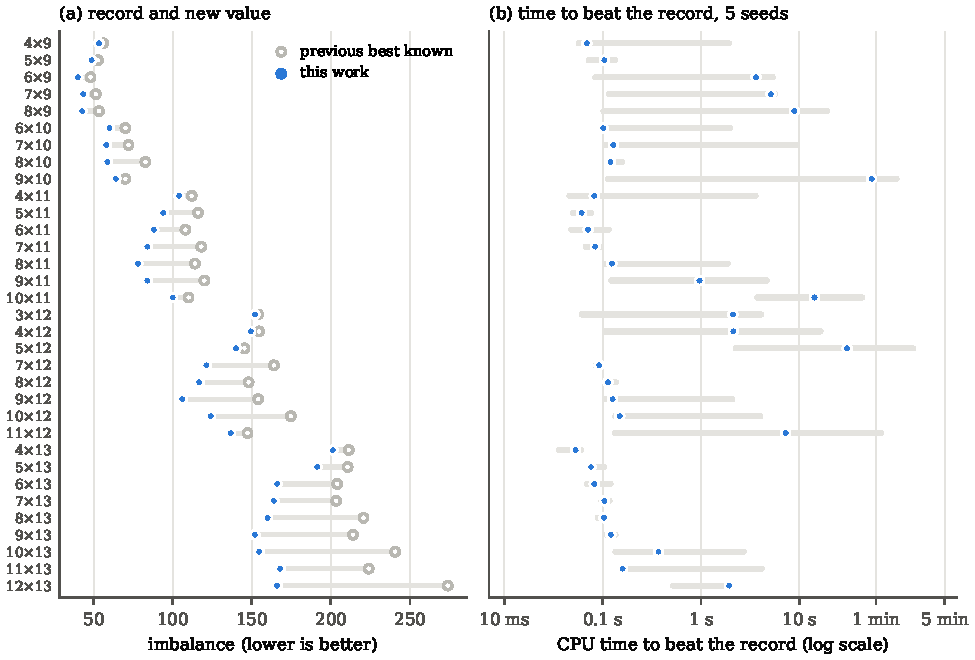
\includegraphics[width=\linewidth]{figures/records_speed.pdf}
\caption{The \NumImproved{} improved instances. (a)~Previous record (open circle) and new value
(filled). (b)~CPU time until the search first beats the record: median (dot) and range (bar)
over \NumSeeds{} seeds, log scale.}
\label{fig:records}
\end{figure}

\section{Why earlier local search stayed in the cyclic orbit}\label{sec:orbit}

\citet{DiazLeBrasGomes2017} note that their local search, which starts from a cyclic
rectangle and permutes columns, ``never leaves its isotopic class''. We make this precise
with an invariant that detects whether a rectangle can come from a group table. It is not a
complete isotopy invariant.

\begin{definition}
The \emph{row group} of a Latin rectangle with rows $r_1,\dots,r_k$ is the permutation group on
symbols
\[
  \row(L)=\bigl\langle\, r_i\circ r_j^{-1} : 1\le i,j\le k \,\bigr\rangle\ \le\ \Sym_n .
\]
\end{definition}

The element $r_i\circ r_j^{-1}$ sends the symbol in column $c$ of row $j$ to the symbol in column
$c$ of row $i$. Since $r_i r_j^{-1}=(r_ir_1^{-1})(r_jr_1^{-1})^{-1}$, the group is already
generated by the $k-1$ ratios $r_ir_1^{-1}$.

\begin{proposition}\label{prop:rowgroup}
\leavevmode
\begin{enumerate}[label=(\roman*),itemsep=1pt]
\item Permuting columns does not change $\row(L)$. Permuting rows permutes its generators.
Relabelling symbols by $\sigma$ replaces it by $\sigma\row(L)\sigma^{-1}$. So the conjugacy
class of $\row(L)$ is an isotopy invariant.
\item If $L$ is isotopic to $k$ rows of the Cayley table of a group $G$ of order $n$, then
$\row(L)$ is conjugate to a subgroup of the left-regular representation of $G$. In particular
it acts semiregularly and $\abs{\row(L)}$ divides $n$.
\item For $i\ne1$, a swap in row $i$ left-multiplies $r_ir_1^{-1}$ by a transposition and fixes
the other generators. A single swap
can therefore enlarge the row group. Starting from a cyclic rectangle, swaps do reach
rectangles with $\row(L)=\Sym_n$, as the data below show.
\end{enumerate}
\end{proposition}

\begin{proof}
(i)~Replacing every row by $r_i\circ\pi$ gives $(r_i\pi)(r_j\pi)^{-1}=r_ir_j^{-1}$. The other
two statements are immediate. (ii)~Up to isotopy, $r_i(c)=\sigma(a_i b_c)$ with $a_i\in G$ and
$c\mapsto b_c$ a bijection onto $G$. Then $r_ir_j^{-1}$ maps $\sigma(a_jb)$ to $\sigma(a_ib)$,
so it is $\sigma\lambda_{a_ia_j^{-1}}\sigma^{-1}$, where $\lambda_g$ is left multiplication by
$g$. (iii)~Swapping two symbols in row $i$ replaces $r_i$ by $\tau r_i$ for a transposition
$\tau$.
\end{proof}

So any search whose moves permute columns, or that selects rows from a cyclic Latin square, stays
among rectangles whose row group is cyclic of order dividing $n$. \Cref{fig:rowgroups} shows
the row groups of the best rectangles we found. Of the \NumImproved{} improved rectangles, 29
have row group $\Sym_n$ and 3 have $\Alt_n$. These are the largest possible groups, as for most random tuples of
permutations~\citep{Dixon1969}, so the
rectangles are as far from any group table as they can be. The exception, $5\times 12$, has a
row group of order $46080=2^6\cdot 6!$, the full centraliser $\Sym_2\wr\Sym_6$ of the pairing
$u\leftrightarrow 13-u$ of
symbols, a mirror symmetry that also appears in the published $4\times12$ and $5\times12$
records.

\begin{figure}[t]
\centering
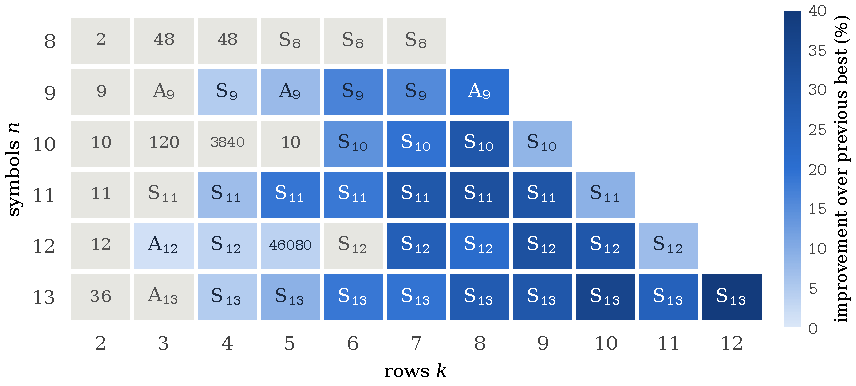
\includegraphics[width=0.92\linewidth]{figures/rowgroups.pdf}
\caption{Row groups of our best rectangles in the benchmark range. Shading shows the improvement
over the previous best value, and grey cells are matched records. Each label gives the row group: $\Sym_n$ or
$\Alt_n$, otherwise its order. Small row groups occur only among matched records.}
\label{fig:rowgroups}
\end{figure}

\paragraph{What this does and does not explain.} The row group explains why rectangles like ours
are unreachable for column-based local search. It does not explain why annealing finds better upper bounds than those reported by the exact
solvers. The SAT and MIP records are also non-cyclic: ten of the fourteen published
rectangles have row group $\Sym_n$. Those methods pursue different goals, proving optimality or learning reusable streamliners, and
we have not isolated which ingredient of our search matters. One plausible factor is
throughput: a move
costs $O(n)$, and the search makes hundreds of millions of them.

\section{Exact search and a new optimum}\label{sec:exact}

To complement the upper bounds, we wrote a branch and bound that decides whether a rectangle
with $3I<B$ exists for a given bound $B$.

\paragraph{Branching.} With $r_1=\mathrm{id}$ fixed, symbols are placed in the order $1,2,\dots,n$.
Placing a symbol means choosing its column in each row $2,\dots,k$, subject to the Latin
conditions. This loses nothing: relabelling symbols turns any rectangle into one with
$r_1=\mathrm{id}$, and relabelling commutes with permuting rows $2,\dots,k$. Among those rows the
columns of symbol $1$ are distinct, so a unique ordering makes them increase with the row index,
and imbalance is invariant under both operations. When symbol $u$ is complete, the deviations $\abs{3d(u,v)-3t}$ for all $v<u$ are final
and are added to the cost.

\paragraph{Bounds.} Two lower bounds prune the tree. First, every unplaced row adds at least $1$
to any distance, because the two symbols occupy different columns. So while a symbol is being
placed, a partial distance that exceeds $t$ even after adding $1$ for each remaining row
contributes a known overshoot, and the node is pruned when the cost so far plus this overshoot
reaches $B$. Second, when a symbol is completed, every pair that is not yet final contributes at
least $m_0=\min(3t\bmod 3,\,3-3t\bmod 3)$ to $3I$, and the node is pruned when the cost plus
$m_0$ times the number of such pairs reaches $B$. For $3\times n$ and $4\times 8$ we have $m_0=0$,
so there the overshoot bound does all the work. Running with $B$ equal to the value of our
rectangle either finds a better rectangle or proves that none exists.

\begin{theorem}\label{thm:3x9}
The minimum imbalance of a $3\times 9$ Latin rectangle is $56$.
\end{theorem}

\noindent The upper bound is the rectangle of \cref{fig:optimum}. The branch and bound
explores $5.5\cdot10^9$ nodes in $140$ CPU seconds and finds no rectangle with $I<56$. Run with
the bound $3I<169$ instead, it finds a rectangle of value $56$, as a sanity check. The value
$56$ itself was already found by~\citet{DiazLeBrasGomes2017}. To our knowledge its optimality
was not known: it is listed as unproven there and in Table~1
of~\citep{VoborilRamaswamySzeider2025}.

\begin{table}[t]
\centering
\small
\begin{tabular}{@{}lrrrl@{}}
\toprule
instance & optimum $I$ & nodes & CPU time & status before this work \\
\midrule
$2\times n$, $n\le 11$ & see \cref{fig:cubic} & $\le 3.8\cdot10^7$ & $\le 1.1$\,s & proven \citep{DiazLeBrasGomes2017,MirkaEtAl2023} \\
$3\times 8$ & 36.0 & $7.8\cdot10^7$ & 1.9\,s & proven \citep{DiazLeBrasGomes2017,RamaswamySzeider2023} \\
$4\times 8$ & 32.0 & $1.9\cdot10^{10}$ & 477\,s & proven \citep{VoborilRamaswamySzeider2025} \\
$3\times 9$ & \textbf{56.0} & $5.5\cdot10^9$ & 140\,s & \textbf{open} \\
\midrule
$5,6,7\times 8$;\ $4$--$8\times 9$ & --- & --- & $>1800$\,s & open (undecided) \\
\bottomrule
\end{tabular}
\caption{Exact branch and bound, single core. Each run proves that no rectangle beats our upper
bound. On all small instances with $n\le7$ and $k\le4$ it also reproduces the values reported
in~\citep{DiazLeBrasGomes2017}.}
\label{tab:exact}
\end{table}

\Cref{tab:exact} summarises the runs. The method is deliberately plain: no symmetry beyond row
order and symbol relabelling, and no learned bounds. It reaches its limit quickly. With a
30-minute cap per instance, the remaining open instances with $n\in\{8,9\}$ stay undecided. Unlike
the DRAT proofs of~\citep{RamaswamySzeider2023}, our search does not emit a checkable
certificate. \Cref{thm:3x9} therefore rests on the correctness of a short program, which we
publish and validated on all the known optima listed above. A DRAT certificate in the style
of~\citep{RamaswamySzeider2023} is the natural next step. The overshoot bound used for pruning
may also be worth encoding there as a redundant constraint.

\section{The cubic law}\label{sec:cubic}

Why does imbalance grow so quickly with $n$ (\cref{tab:results}), and why can squares be perfectly
balanced? The point picture gives a short answer. For fixed $k$, there is not enough room in
$[n]^k$ for $n$ points that are pairwise far apart.

\begin{theorem}\label{thm:cubic}
Let $L$ be a $k\times n$ Latin rectangle and $s\ge 1$ an integer, and put
$B=\ceil{n/s}^k$. Then
\[
  I(L)\ \ge\ n\Bigl(\frac nB-1\Bigr)\Bigl(\frac{k(n+1)}3-k(s-1)\Bigr)
\]
whenever both brackets are positive. Consequently, for every fixed $k$,
\[
  c_k\ \le\ \liminf_{n\to\infty}\frac{\min I}{n^3}\ \le\ \limsup_{n\to\infty}\frac{\min I}{n^3}\ \le\ \frac k3,
  \qquad
  c_k=\max_{m\ge 4}\ \frac{k}{m^k}\Bigl(\frac13-\frac1m\Bigr)>0 .
\]
\end{theorem}

\begin{proof}
Cut each axis of $[n]^k$ into $\ceil{n/s}$ intervals of at most $s$ consecutive values. This
cuts the grid into $B$ boxes. Two points in the same box differ by at most $s-1$ in every
coordinate, so their distance is at most $k(s-1)<t$. If box $b$ holds $m_b$ of the $n$ points,
convexity gives
\[
  \sum_b\binom{m_b}{2}\ \ge\ B\binom{n/B}{2}=\frac n2\Bigl(\frac nB-1\Bigr)
\]
pairs that share a box. Each of them has $t-d\ge t-k(s-1)$. Inserting this
into~\eqref{eq:half} proves the first claim. For the second, take $s=\ceil{n/m}$ for a
fixed $m$. Then $B\le m^k$ and $s-1<n/m$, and the bound becomes
$k\,m^{-k}(\frac13-\frac1m)\,n^3-O(n^2)$. For the upper bound, $k\le d\le k(n-1)$ gives
$\abs{d-t}\le\frac{2k(n-2)}3$, and $\binom n2\cdot\frac{2kn}{3}\le\frac{k n^3}{3}$.
\end{proof}

The proof is a pigeonhole argument, and \cref{fig:geometry}a shows it at work. Clustered points
are expensive, and in a low-dimensional grid clustering is unavoidable. Three remarks put the
theorem in context.

\begin{remark}[Constants]
For $k=2$ the maximum is attained at $m=5$, giving $c_2=4/375\approx0.0107$. For $k\ge3$,
$c_k=k/(12\cdot4^k)$, attained at $m=4$. In the benchmark range the finite-$n$ bound is weak: for $2\times13$
it gives $7.7$, against the true optimum $218.6$, and for $k=3$ it becomes positive only at
$n=28$. Its message is asymptotic. Even the \emph{average} deviation per pair, $I/\binom n2$, grows linearly in $n$, the
same order as the target $t$ itself. For fixed $k$, rectangles are not merely imperfect but
\emph{uniformly} imperfect.
\end{remark}

\begin{remark}[Squares]
The bound is useless when $k$ grows with $n$, and it must be, because spatially balanced Latin
squares exist, for instance whenever $2n+1$ is prime, by a construction that was itself
discovered through streamlined search~\citep{LeBrasGomesSelman2012}. In $[n]^n$ there is room for $n$ equidistant points.
\end{remark}

\begin{remark}[Equilateral sets]\label{rem:equilateral}
A perfectly balanced rectangle is a set of $n$ points in $\R^k$ that are pairwise equidistant in
$\ell_1$, an \emph{equilateral set} of $\ell_1^k$. Hence $n\le e(\ell_1^k)$, the largest size of
such a set. Kusner conjectured $e(\ell_1^k)=2k$, which is known for
$k\le4$ (the case $k=4$ is due to \citet{KoolenLaurentSchrijver2000}; see~\citep{Swanepoel2004}),
and \citet{AlonPudlak2003} proved
$e(\ell_1^k)=O(k\log k)$ in general (see also the survey~\citep{Swanepoel2004}). So a perfectly
balanced $k\times n$ rectangle needs $k=\Omega(n/\log n)$ rows. For $k\le4$ this gives
$n\le2k$, which recovers part of the case analysis of~\citet{DiazLeBrasGomes2017}. Their
arguments are sharper for $k\le 3$, and their bound $k\ge 6-18/(n+1)$ coincides with ours at
$k=4$, while theirs is vacuous for $k\ge6$. The point sets of rectangles are far more special than general equilateral sets, since
their coordinate projections are bijections onto $[n]$, so we do not expect these bounds to be
tight. We have not seen this connection made in the literature on balanced designs.
\end{remark}

\section{Two rows}\label{sec:two}

For $k=2$ a rectangle is a permutation $\pi=r_2$ together with the fact that it has no fixed
points, and the points $x_u=(u,\pi^{-1}(u))$ form its permutation diagram. \citet{MirkaEtAl2023}
solved $n\le13$ to optimality with a clique-based MIP and reported bounds up to $n=20$ after six
hours. \Cref{tab:two} adds our two-minute annealing runs. They improve the upper bound for
$15\le n\le 19$, tie at $n=14$ and lose at $n=20$, where the best bound of~\citep{MirkaEtAl2023}
came from eight parallel six-hour runs. These are single runs with one seed, the improvements are
small ($0.2$--$2\%$), and the MIP also spends its time on lower bounds, so the comparison shows
only that annealing is a strong source of incumbents. The lower bounds remain far away, and we have not attempted to improve them.

\begin{table}[t]
\centering
\small
\begin{tabular}{@{}lrrrrrrr@{}}
\toprule
$n$ & 14 & 15 & 16 & 17 & 18 & 19 & 20 \\
\midrule
lower bound \citep{MirkaEtAl2023} & 201.57 & 252.6 & 273.82 & 252.0 & 402.6 & 465.3 & 155.0 \\
upper bound \citep{MirkaEtAl2023} & 268.0 & 345.3 & 427.3 & 508.0 & 617.3 & 732.0 & 816.0 \\
annealing (this work)             & 268.0 & \textbf{344.6} & \textbf{422.0} & \textbf{498.0} & \textbf{610.6} & \textbf{722.6} & 832.0 \\
\bottomrule
\end{tabular}

\caption{$2\times n$ rectangles beyond the proven range. The lower and upper bounds are the best
over all methods and configurations in~\citep{MirkaEtAl2023}, from 6-hour runs. Annealing:
one 2-minute single-core run. Bold: better than the previous upper bound. The lower bounds are
those reached when the 6-hour limit expired, which is why they are not monotone in $n$.}
\label{tab:two}
\end{table}

\begin{figure}[t]
\centering
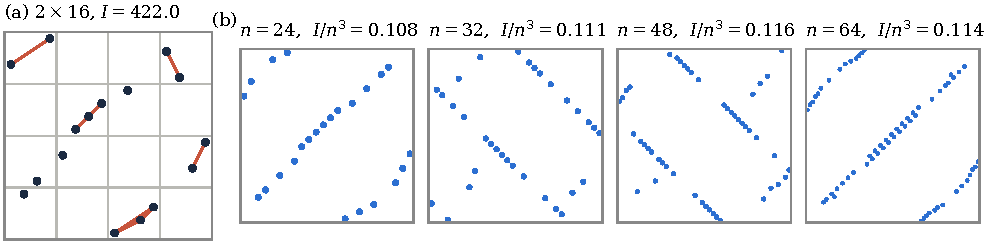
\includegraphics[width=\linewidth]{figures/geometry.pdf}
\caption{$2\times n$ rectangles as point sets. (a)~The proof of \cref{thm:cubic} for a
$2\times16$ rectangle with $I=422$: a $4\times4$ grid of boxes, and in red the pairs that share
a box. Each such pair is closer than the average $t=34/3$ and costs imbalance.
(b)~The best rectangles found by annealing for larger $n$ (one 2-minute run each), rescaled to
the unit square. Most points lie on a few long parallel diagonal runs, with scattered extra
points.}
\label{fig:geometry}
\end{figure}

\begin{figure}[t]
\centering
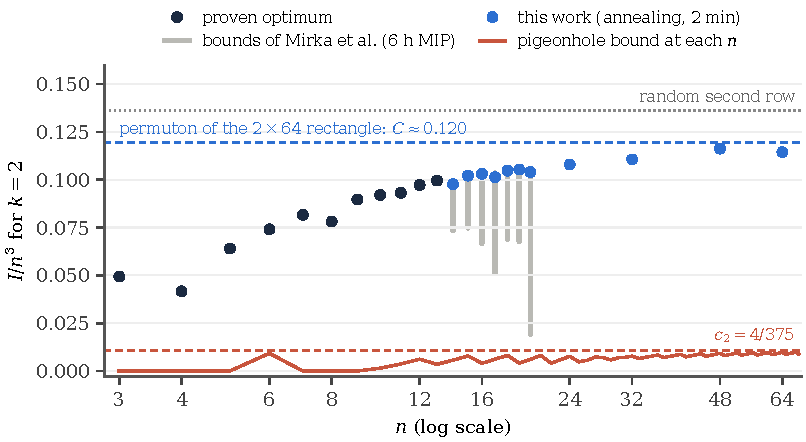
\includegraphics[width=0.9\linewidth]{figures/cubic.pdf}
\caption{Normalised imbalance $I/n^3$ for $k=2$. Black: proven optima. Grey: interval between
the best lower and upper bounds of~\citep{MirkaEtAl2023}. Blue dots: our annealing values; blue dashes: $C(\mu_\sigma)$ for our $2\times64$ rectangle,
an upper estimate for the limit (\cref{prop:limit}). Red:
\cref{thm:cubic} at each $n$ (solid) and its limit $c_2$ (dashed). A uniformly random
derangement has $I/n^3\to0.1361$ (dotted).}
\label{fig:cubic}
\end{figure}

\paragraph{The shape of optimal permutations.} \Cref{fig:geometry}b shows the best permutations
that annealing finds for $n=24,\dots,64$. They are far from random. Most points lie on a few
long parallel segments of slope $1$, cyclically shifted against one another, with a minority of
scattered points.

\paragraph{A limit object.} A \emph{permuton} is a probability measure on $[0,1]^2$ with
uniform marginals. Every permutation $\sigma$ of $[n]$ defines one, $\mu_\sigma$, uniform on
the squares $[\frac{i-1}n,\frac in]\times[\frac{\sigma(i)-1}n,\frac{\sigma(i)}n]$. Put
\[
  C(\mu)=\tfrac12\,\mathbb E\,\bigl|\,\abs{X-X'}+\abs{Y-Y'}-\tfrac23\,\bigr|,
\]
where $(X,Y)$ and $(X',Y')$ are independent samples of $\mu$.

\begin{proposition}\label{prop:limit}
For $k=2$, $\min I/n^3$ converges as $n\to\infty$ to $\min_\mu C(\mu)$, where the minimum over
permutons is attained.
\end{proposition}

\begin{proof}[Proof sketch]
The integrand is bounded and continuous on $[0,1]^4$, so $C$ is continuous for the weak topology.
Permutons form a compact set, so the minimum is attained. For any permutation $\sigma$, comparing the sum defining $I$ with the integral defining $C(\mu_\sigma)$ cell by cell (the $n$
diagonal cells, absent from $I$, have total weight $1/n$)
gives $I/n^3=C(\mu_\sigma)+O(1/n)$, because the integrand is Lipschitz and $t/n\to\frac23$.
This yields $\liminf\min I/n^3\ge\min C$. Conversely, permutations $\sigma_n$ with
$\mu_{\sigma_n}\to\mu$ exist for every permuton $\mu$ (sample $n$ points from $\mu$; see~\citep{HoppenEtAl2013}). Removing
fixed points by swapping each with an adjacent column, which never creates a new fixed point,
changes $I$ by $O(n)$ per fixed point, so by
$O(n^2)$ in total, which gives the matching upper bound.
\end{proof}

The uniform permuton gives $C=496/3645\approx0.1361$, the limit for a random derangement, and the
diagonal (the cyclic rectangle) gives $16/81\approx0.198$. Optimising numerically over permutons
made of $m$ increasing or decreasing segments gives $0.148$, $0.133$ and $0.124$ for $m=3,4,5$.
The permuton of our $2\times64$ rectangle does better, with $C(\mu_\sigma)\approx0.120$ by numerical
quadrature, and this is our best estimate from above for the limit. The finite values
$I/n^3\approx0.11$ in \cref{fig:cubic} lie below it mainly because the diagonal cells add a
positive $O(1/n)$ term to $C(\mu_\sigma)$, so as estimates of the limit
they are biased low by roughly $c/n$.

\begin{question}
What is $\lim_n\min I(2\times n)/n^3=\min_\mu C(\mu)$? We know only that it lies between
$4/375\approx0.011$ and about $0.120$. Is the minimiser unique, and is it a finite union of
segments?
\end{question}

\section{Discussion}

The three parts of this paper inform one another. The point picture says that balance is a
packing problem in $\ell_1$, so moving points is the natural move. The row group says that moves
which only shuffle columns cannot leave a cyclic orbit, while within-row swaps can reach rectangles
whose row group is all of $\Sym_n$. The cubic law gives the right scale. Imbalance is not a
small defect that clever search will remove, but a quantity of order $n^3$ whose leading
constant is the real object of study.

\paragraph{Limitations.} The new upper bounds come from one run per instance and budget, so
the search is not a controlled experiment. We did not isolate the effect of the adaptive penalty
or rerun earlier local search head-to-head. We make no runtime comparison with earlier work. The
optimality of $3\times 9$ rests on an uncertified program. Our lower-bound theorem is far from
the observed values for $k=2$ and is negligible in the benchmark range.

\paragraph{Open problems.} (1)~Certify \cref{thm:3x9}, for instance with a DRAT-producing SAT
encoding as in~\citep{RamaswamySzeider2023}, and settle $5\times8$ to $7\times8$. Our new upper
bounds are natural starting incumbents for certified solvers, and the mirror pairing
$u\leftrightarrow n+1-u$ seen in several records is a candidate streamliner in the sense
of~\citep{VoborilRamaswamySzeider2025}. (2)~Close the gap
between $c_2=0.0107$ and $0.120$. A sharper lower bound might weight pairs by distance instead of
counting close pairs in boxes. (3)~Determine the minimising permuton for $k=2$.
(4)~Prove Kusner's conjecture for $\ell_1$, which would show that perfectly balanced
$k\times n$ rectangles need $k\ge n/2$.

\paragraph{Data and code.} Rectangles, the annealing code, the branch and bound, the exact
checker and the scripts for every figure are at
\\\url{https://github.com/BrianLi009/Balanced-Latin-Rectangles}.

\FloatBarrier
\bibliographystyle{plainnat}
\bibliography{refs}

\end{document}
